\chapter{Implementation}
\label{chapter:implementation}
% \epigraph{The best presents don't come in boxes.}{Bill Watterson}
% \epigraph{Typing is no substitute for thinking.}{Dartmouth Basic manual, 1964}

This chapter is divided into two parts.
The first half of this chapter will describe the execution of TASTy trees in a Truffle interpreter.
The second half of this chapter covers the techniques we will use to eliminate autoboxing Truffle itself is unable to eliminate. 

\section{Execution}

Scala programs in \acrshort{tasty} format are unsuitable for execution in a Truffle interpreter. 
Programs in must be parsed and transformed into an executable representation in \textsc{TastyTruffle}. 
As TASTy represents a Scala program close to its equivalent source representation, canonicalization compiler passes (see appendix \ref{appendix:dotty-phases}) that would otherwise normalize the IR are not present. 
Instead, we implement TastyTruffle IR to represent a canonicalized executable intermediate representation which can be specialized on demand. 

In the following sections, we will describe the features of TASTy and why it is directly unsuitable for execution and how to simplify their nodes into TastyTruffle IR.
We will begin with a explanation of how data is encoded and defined in TASTy.

\subsection*{Types}

Types are a set of properties and rules for reasoning about the behaviour of programs. 
In the Scala type system, types can be distinguished between \textit{value types} and \textit{type constructors}. 
Value types refer to the definition of a \textit{class}. 
Type constructors accept type parameters as arguments and produce a resulting type.

\subsection{Generating Frame Slots from \texttt{ValDef} trees} 

The \scalainline{ValDef} tree is a multi-purpose node which represents value definitions in many contexts.
This section will only cover the \scalainline{ValDef} tree in the context of local variables.
Sections \ref{impl:subsection:defdef} and \ref{impl:subsection:classdef} will cover the remaining contexts in which \scalainline{ValDef} trees appear.

Local variables are variables which are bound to a \textit{scope}. 
A scope represents the lifetime in which a variable can refer to an entity. 
Similarly, uses of variables are only valid when used under the appropriate scope. 
Local variables and their use sites are represented in intermediate representations through a myriad of methods. 
In abstract syntax trees, local variables and their used are represented as nodes \textit{dominated} by their scopes (which are themselves nodes). 
Unlike more simplified \acrshort{ir}, abstract syntax trees do not encode any data dependence between definitions and uses\cite{ssa}. 
In order to execute the tree, name binding must be resolved when ???

In \acrshort{tasty}, a local variable is represented by the \scalainline{ValDef} tree node:

\begin{figure}[H]
	\begin{minted}{scala}
		case class ValDef(name: String, tpt: TypeTree, rhs: Option[Term]) extends Tree 
	\end{minted}
	\caption{Simplified \scalainline{ValDef} tree}
\end{figure}

The \scalainline{ValDef} tree represents the site of a local variable declaration when the node is dominated by a \scalainline{Block} node. 
A \scalainline{ValDef} contains the simple, unqualified name of the declaration, the type as represented in the source program and the intializer. 
When a \scalainline{ValDef} is owned by a \scalainline{Block}, the initializer will always be non-empty.

Each unique variable declaration has a corresponding frame slot in the frame descriptor of its root node. 
Truffle permits each frame slot in a frame descriptor be described by a \textit{frame slot kind}.
At the time of writing, a frame slot kind can be implemented as:

\begin{figure}[H]
	\begin{minted}{scala}
		object FrameSlotKind extends Enumeration {
			type FrameSlotKind = Value
			val Object, Long, Int, Double, Float, Boolean, Byte = Value
		}
	\end{minted}
	\caption{Simplified implementation of \scalainline{FrameSlotKind}}
\end{figure}

There is a corresponding frame slot kind for each \acrshort{jvm} primitive and reference types. 
We determine the frame slot kind of a type using the following method:

\begin{figure}[H]
	\begin{minted}{scala}
		def getFrameSlotKind(tpe: Type): Option[FrameSlotKind] = {
			if (tpe.isMonomorphic && tpe.isPrimitive)
			Some(primitiveSlotKindOf(tpe))
			else if (tpe.isParameter)
			None
			else
			Some(FrameSlotKind.Object)
		}	
	\end{minted}
	\caption{Pseudocode for determining the frame slot kind of a type.}
\end{figure}

Truffle specializes local variable access based on the variable's type during partial evaluation\cite{truffle:partial-eval}. 
To eliminate the need to specialize read and writes of variables where types are monomorphic and statically refer to a primitive type, the primitive frame slot kind is matched in the frame descriptor. 
In all other cases, including when the type is not resolvable through a single type parameter, e.g. \scalainline{val x: T}, we assign the frame slot the \scalainline{Object} frame slot kind.
We will defer discussion of variable declarations which have polymorphic types that cannot be resolved statically until section \ref{implementation:specialization}.

\subsection{The \texttt{DefDef} tree}
\label{impl:subsection:defdef}

\subsection{Deriving Shapes from the \texttt{ClassDef} Tree}
\label{impl:subsection:classdef}

In object oriented programming languages, \textit{objects} are instances of a class.

\begin{figure}[!htb]
	\begin{minted}{scala}
	private ClassShape(
		symbol:  Symbol,
		parents: Array[Symbol],
		fields:  Array[Field] ,
		methods: Map[MethodSignature, RootCallTarget]
		vtable:  Map[Signature, Symbol]
	)
	\end{minted}
	\caption{Simplified implementation of a shape.}
\end{figure}

\subsection{The \texttt{Assign} tree}

\subsection{Initializing Objects with the \texttt{New} Tree}

\subsubsection{Escape Analysis}

Escape analysis\cite{escape-analysis} reasons about the dynamic scope of object allocations. 
Compiler implementations often exploit the observations of escape analysis to enable optimizations such:

\begin{description}
	\item[Region Allocation\cite{java:escape-analysis}\cite{tofte:region-memory}] The substitution of heap allocations with stack allocations to eliminate unnecessary garbage collection.
	\item[Scalar Replacement\cite{java:escape-analysis-optimizations}] The complete elimination of an object allocation, where the fields of the replaced object are substituted by local variables.
\end{description}

GraalVM employs \textit{Partial Escape Analysis}\cite{java:partial-escape-analysis}, a path-sensitive variant of escape analysis which is particularly effective when combined with optimizations described above as well other compiler optimization such as inlining. 
Truffle offers guest language implementations the \scalainline{VirtualFrame} abstraction to allow guest language semantics to take advantage of partial escape analysis and subsequent optimizations.

\subsection{The \texttt{Block} tree}

\subsection{The \texttt{While} tree}

\subsection{The \texttt{Select} tree}

% Intro

\subsection{The \texttt{Apply} tree}


As previously mentioned, method invocations exists in multiple forms because tree canocalization happens immediately after the TASTy picking phase in the compilation pipeline.
The result is that TASTy trees retain some syntactic elements from their Scala sources. 
For example, Truffle provides two abstractions for call nodes, the \textit{direct call node} is used when the call target can be statically resolved. 
In TASTy, this includes the set of methods with private or final modifiers\cite{java:lang-spec} and class constructors. 
Otherwise, the \textit{indirect call node} is used for calls which have dynamically resolved call targets. 
\textsc{TastyTruffle} uses a singular call node implementation for both monomorphic and polymorhic calls. 
we utilize a polymorphic inline cache\cite{self:polymorphic-inline-caches} to eliminate the overhead of resolving polymorphic calls for \acrshort{jit} compilation. 
Figure \ref{implementation:poly-cache-call-node} shows a simplified Truffle call node in \textsc{TastyTruffle} which implements a polymorphic inline cache.

\begin{figure}[!htb]
	\begin{minted}{scala}
	class ApplyNode(sig: Signature, receiver: TermNode, args: Array[TermNode]) extends TermNode {
		
		final val INLINE_CACHE_SIZE: Int = 5;
		
		@Specialization(guards = "inst.type == tpe", limit = "INLINE_CACHE_SIZE")
		def cached(
			frame: VirtualFrame,
			inst: ClassInstance,
			@Cached("inst.type") tpe: Type,
			@Cached("create(resolveCall(instance, sig)") callNode: DirectCallNode
		): Object = callNode.call(evalArgs(frame, inst));
		
		@Specialization(replaces = "cached")
		def virtual(
			frame: VirtualFrame,
			inst: ClassInstance,
			@Cached callNode: IndirectCallNode
		): Object = {
			val callTarget = resolveCall(instance, sig);
			callNode.call(callTarget, evalArgs(frame, inst))
		}
	}
	\end{minted}
	\caption{Simplified implementation of the call node with a polymorphic inline cache used in TastyTruffle.}
	\label{implementation:poly-cache-call-node}
\end{figure}

The Truffle \acrshort{dsl} emits a cache which is searched linearly based on the type of receiver. 
When the type of receiver has not been seen in the inline cache, an additional cache entry is generated and appended to the cache for the next call. 
The size of an polymorphic inline cache must be kept reasonable ???. 
The generated inline cache can be used to inline code and JIT optimized based on the type of the receiver seen at a call site. 


\begin{figure}[H]
	\centering
	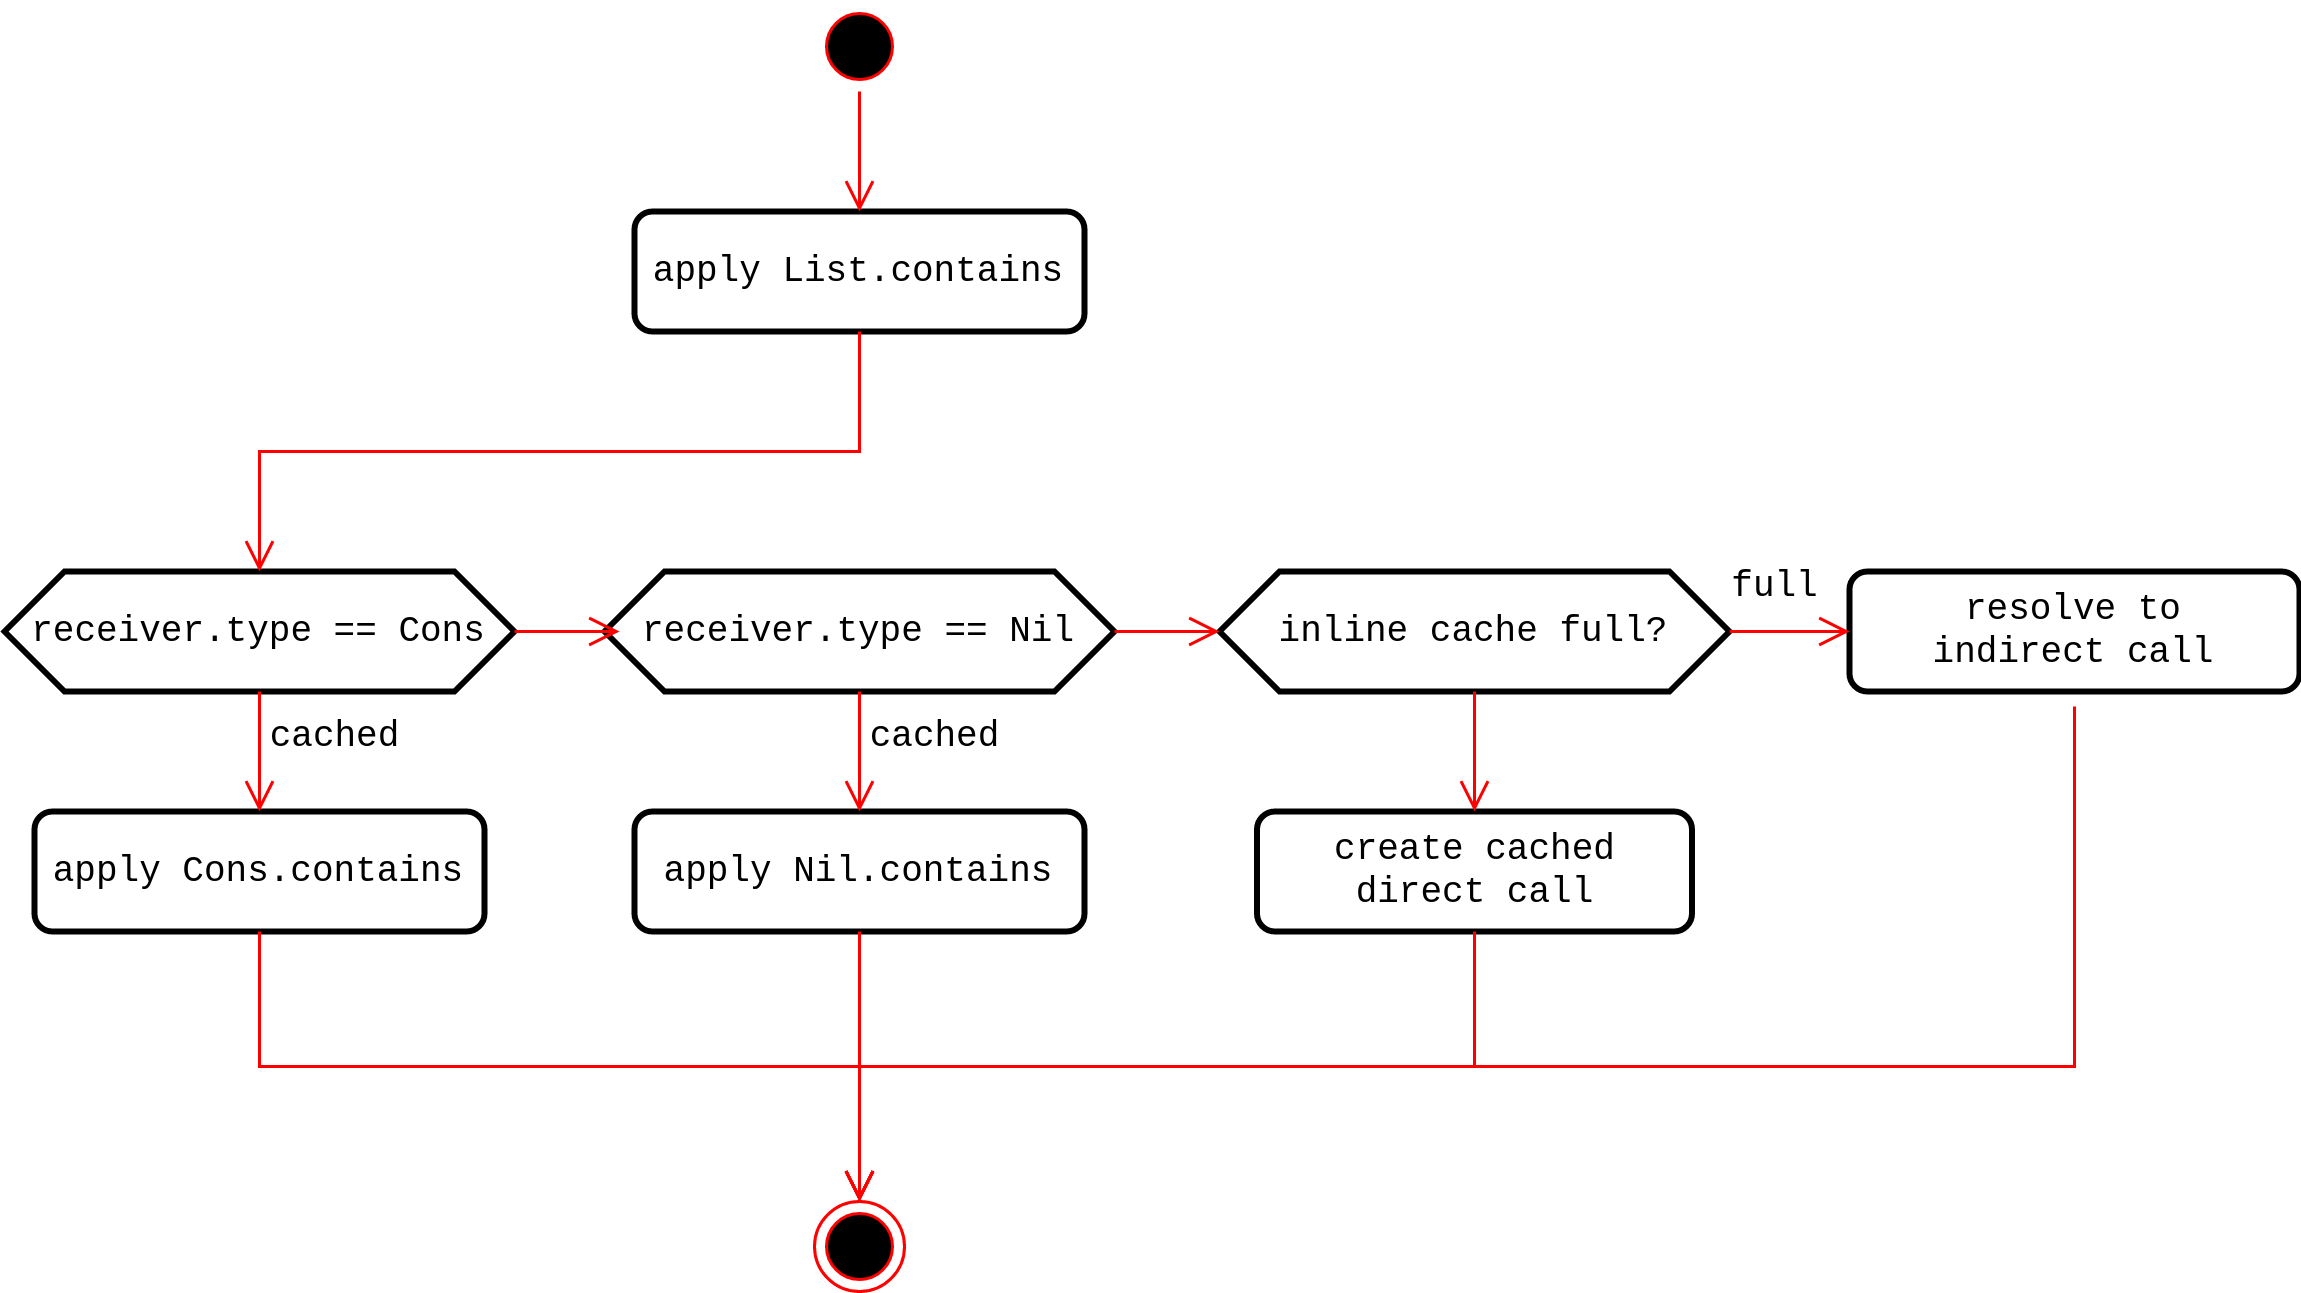
\includegraphics[width=0.75\textwidth]{figures/tastytruffle-pic-example.png}
	\caption{A possible polymorphic inline cache for a \scalainline{List.contains} callsite.}
	\label{example:poly-cache-call-node}
\end{figure}

When the polymorphic inline cache is applied to a monomorphic call site, it simplifies to a single element inline cache\cite{smalltalk:inline-caches}. 
Because the type of the receiver at the call site remains stable, the cache look up of the call target based on the type always succeeds and the call site never fallbacks to using an indirect call node.


\subsubsection{Unary and Binary Expressions}

Unary and Binary operations in Scala are syntactic sugar for function invocation. 
For example, the following addition \scalainline{1 + 2} is desugared to \scalainline{1.+(2)}. 
That is, the binary operator \scalainline{+} is represented as the invocation of the instance function \scalainline{Int.+} on the receiver with value \scalainline{1} and type \scalainline{Int} with a single argument \scalainline{2}.
Normally in the Scala compilation pipeline, methods which operate on primtive types and have an underlying implementation on the JVM\cite{java:vm-spec}, e.g. in a bytecode instruction, are replaced by those instructions in compiled program bytecode. 
Similarly, TastyTruffle avoids implementing methods of primitive types with actual call semantcs as primitive operations are frequently used and simple to optimize as instrinsic implementations exist on many Java virtual machines.\cite{???}


\subsection{The \texttt{Ident} tree}

\section{Specialization}
\label{implementation:specialization}

\subsection{}

\subsection{Specializing Object Layout with \texttt{Applied} type trees}

\begin{figure}[!htb]
	\begin{minted}{scala}
	trait PolymorphicTermNode extends TermNode {
		def resolveType: ClassType 
		override def execute(frame: VirtualFrame): Object = 
			throw new UnsupportOperationException("generic code cannot be executed!")
	}
	\end{minted}
	\caption{A placeholder node for polymorphic code in \textsc{TastyTruffle}}
\end{figure}


\subsection{Specializing Call Sites with \texttt{TypeApply} trees}

Generic methods in Scala can be polymorphic under class type parameters, method type parameters, or both. 
In the latter two cases, polymorphic methods contain additional reified type parameters. 
In addition to the polymorphic terms present in the method body discussed in the previous section, the type of method term parameters may be polymorphic. 
The following components of a generic method must specialized:

\begin{itemize}
	\item Polymorphic method parameters.
	\item Polymorphic terms inside the method body.
\end{itemize}


\subsubsection*{Method Parameters}

\subsubsection*{Typed Dispatch Chains}

Dispatch chains\cite{???}

\begin{figure}[H]
	\begin{minted}{scala}
	class TypeDispatchNode(parent: RootNode) extends TermNode {
		
		type TypeArguments: Array[Type]
		@CompilerDirectives.CompilationFinal
		var cache: Map[TypeArguments, DirectCallNode]
		
		override def execute(frame: VirtualFrame): Object = {
			val types: TypeArguments = resolveTypeParameters(frame)
			dispatch(frame, args);
		}
		
		def dispatch(frame: VirtualFrame, types: TypeArguments): Object = cache.get(types) match {
			case Some(callNode) => callNode.call(frame.getArguments)
			case None => createAndDispatch(frame, types)
		}
		
		def createAndDispatch(frame: VirtualFrame, types: TypeArguments): Object = {
			CompilerDirectives.transferToInterpreterAndInvalidate()
			val specialization = parent.specialize(types)
			val callNode = DirectCallNode.create(specialization)
			cache = cache.updated(types, callNode)
			callNode.call(frame.getArguments)
		}
	}
	\end{minted}
\caption{Simplified implementation of generic dispatch node based on reified type arguments.}
\end{figure}

\begin{figure}[H]
	\centering
	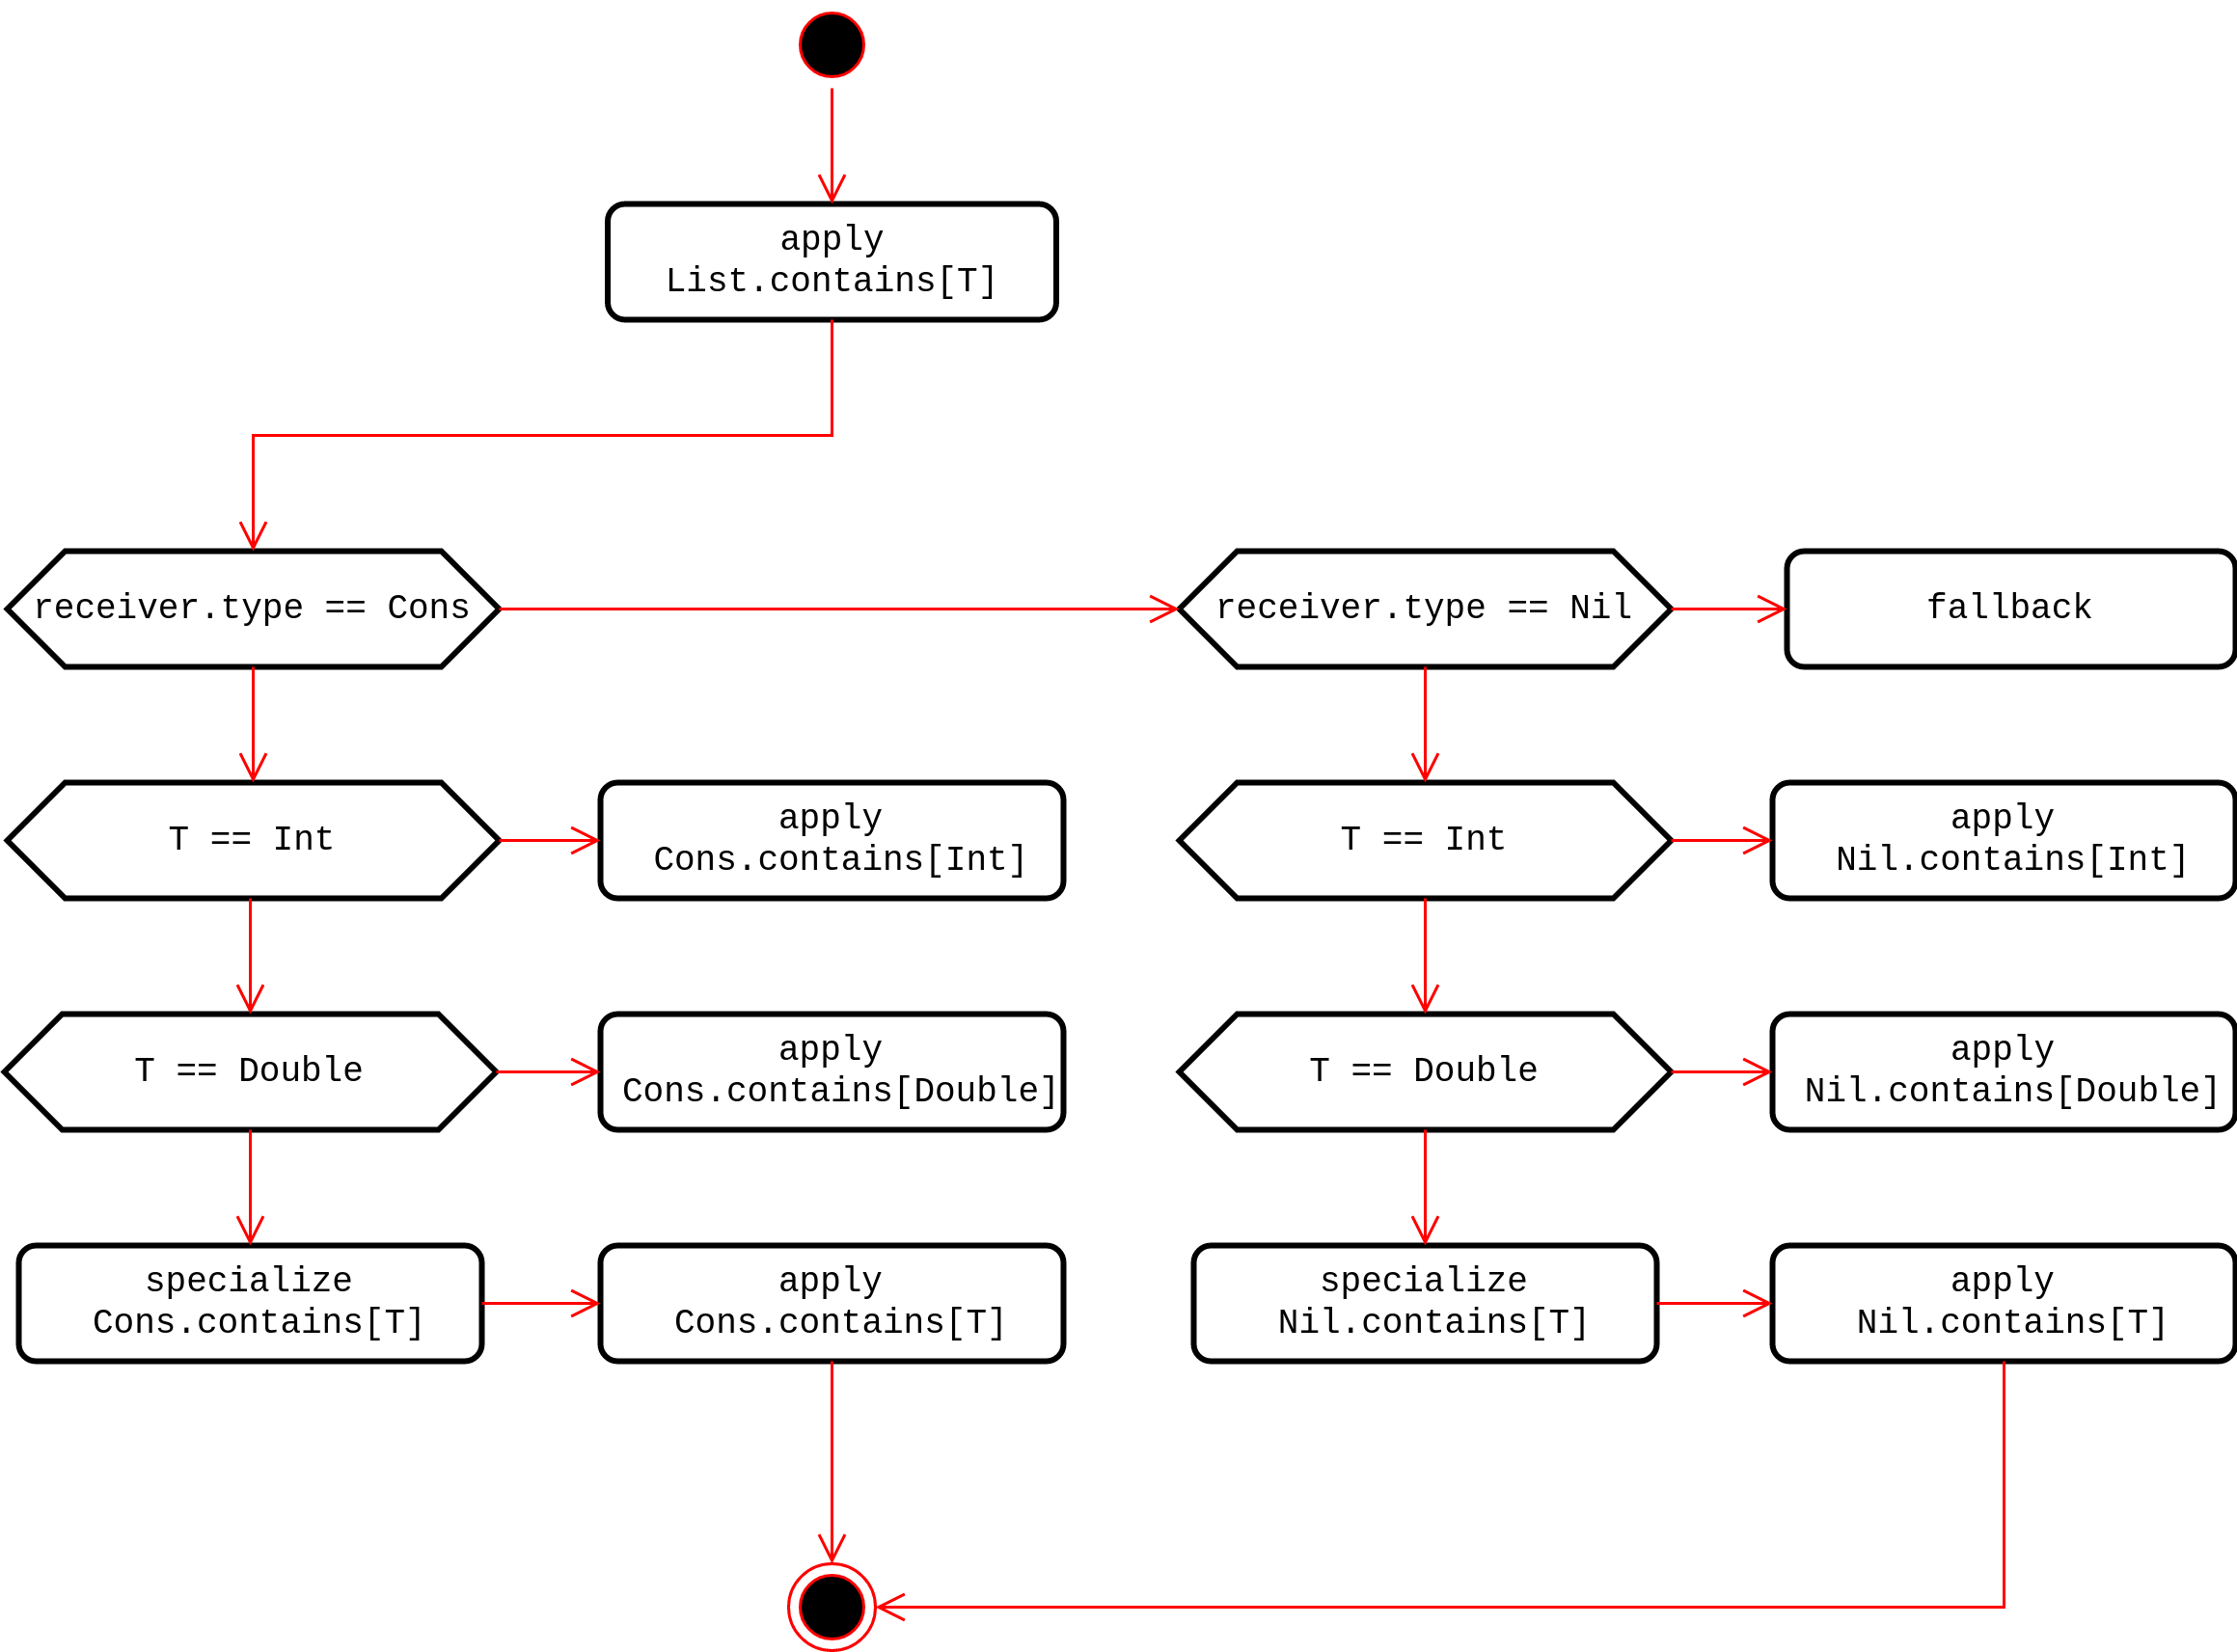
\includegraphics[width=0.75\textwidth]{figures/tastytruffle-type-dispatch-chain.png}
	\caption{The typed dispatch chain for a \scalainline{List.contains} call site }
\end{figure}

\subsubsection*{Code Duplication}

\subsubsection*{Partial Evaluation}

\subsection{Specializing Terms}

\begin{figure}[H]
	\centering
	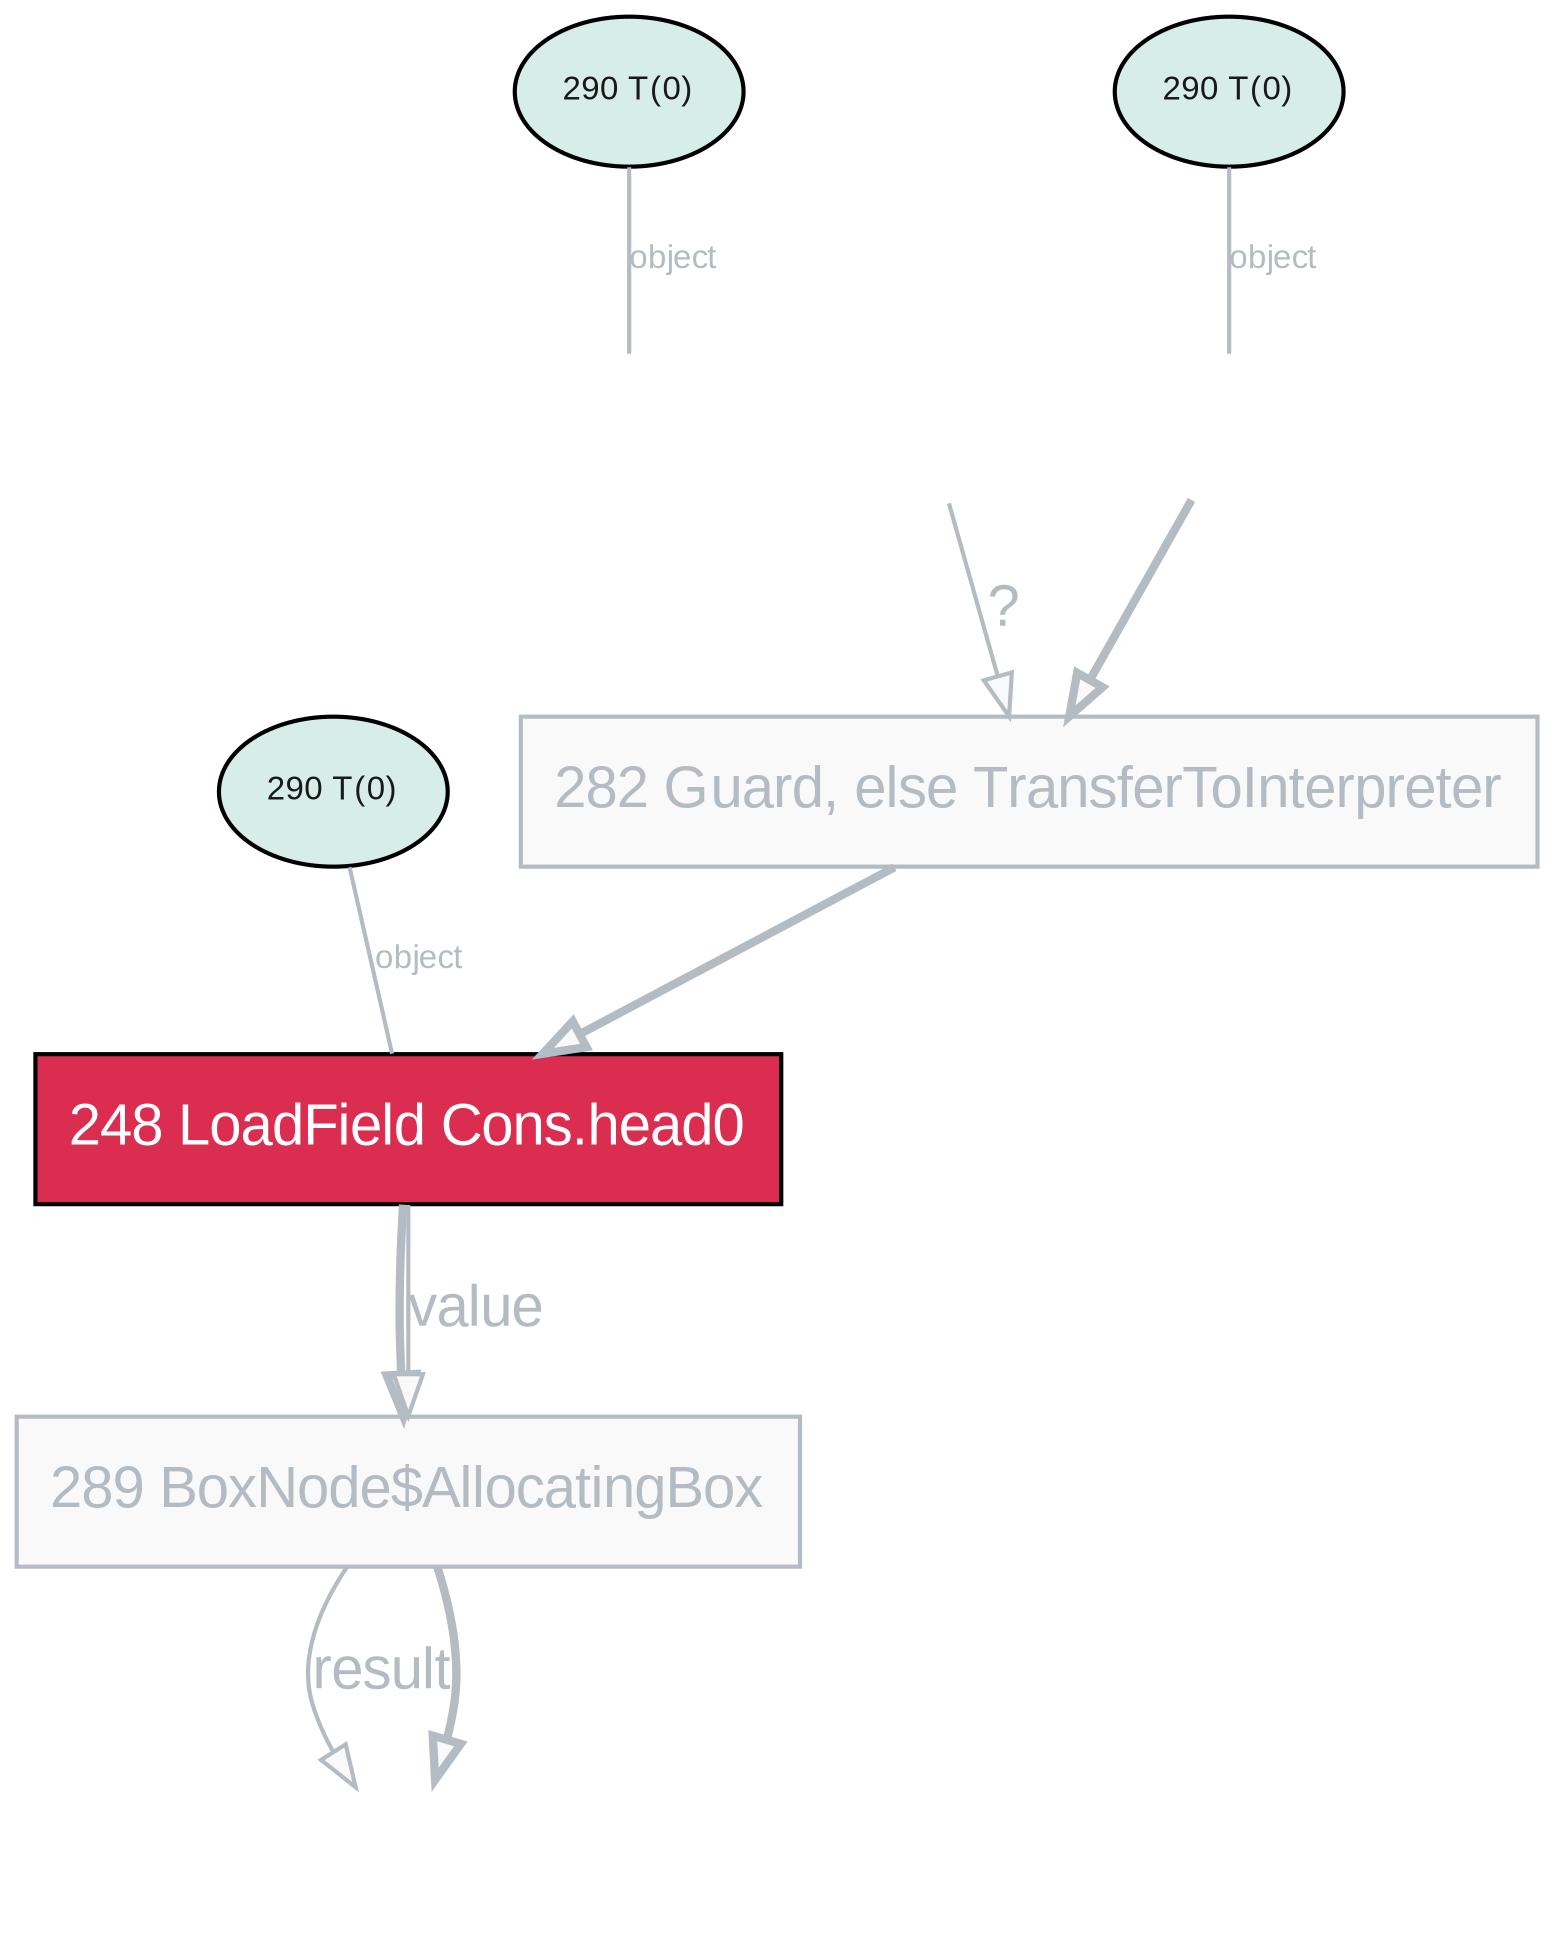
\includegraphics[width=0.35\textwidth]{figures/dot/List.head.TruffleTier.png}
	\caption{Graal IR of \scalainline{List.head} after field read of \scalainline{head0} is specialized.}
\end{figure}

The basic polymorphic unit of code in Scala are terms whose types are derived directly from a type parameter \mintinline{scala}|T| or indirectly from a type constructor such as \mintinline{scala}|Array[T]|.
Polymorphic terms can be divided into the following categories:

\subsubsection*{Polymorphic local access}
\subsubsection*{Polymorphic field access}
\subsubsection*{Polymorphic method call}
\subsubsection*{Polymorphic instantiation}

